% Options for packages loaded elsewhere
\PassOptionsToPackage{unicode}{hyperref}
\PassOptionsToPackage{hyphens}{url}
%
\documentclass[
]{article}
\usepackage{lmodern}
\usepackage{amssymb,amsmath}
\usepackage{ifxetex,ifluatex}
\ifnum 0\ifxetex 1\fi\ifluatex 1\fi=0 % if pdftex
  \usepackage[T1]{fontenc}
  \usepackage[utf8]{inputenc}
  \usepackage{textcomp} % provide euro and other symbols
\else % if luatex or xetex
  \usepackage{unicode-math}
  \defaultfontfeatures{Scale=MatchLowercase}
  \defaultfontfeatures[\rmfamily]{Ligatures=TeX,Scale=1}
\fi
% Use upquote if available, for straight quotes in verbatim environments
\IfFileExists{upquote.sty}{\usepackage{upquote}}{}
\IfFileExists{microtype.sty}{% use microtype if available
  \usepackage[]{microtype}
  \UseMicrotypeSet[protrusion]{basicmath} % disable protrusion for tt fonts
}{}
\makeatletter
\@ifundefined{KOMAClassName}{% if non-KOMA class
  \IfFileExists{parskip.sty}{%
    \usepackage{parskip}
  }{% else
    \setlength{\parindent}{0pt}
    \setlength{\parskip}{6pt plus 2pt minus 1pt}}
}{% if KOMA class
  \KOMAoptions{parskip=half}}
\makeatother
\usepackage{xcolor}
\IfFileExists{xurl.sty}{\usepackage{xurl}}{} % add URL line breaks if available
\IfFileExists{bookmark.sty}{\usepackage{bookmark}}{\usepackage{hyperref}}
\hypersetup{
  pdftitle={Species Distribution Model on Saguaro (Carnegiea gigantea)},
  pdfauthor={Katherine Castrillon},
  hidelinks,
  pdfcreator={LaTeX via pandoc}}
\urlstyle{same} % disable monospaced font for URLs
\usepackage[margin=1in]{geometry}
\usepackage{graphicx,grffile}
\makeatletter
\def\maxwidth{\ifdim\Gin@nat@width>\linewidth\linewidth\else\Gin@nat@width\fi}
\def\maxheight{\ifdim\Gin@nat@height>\textheight\textheight\else\Gin@nat@height\fi}
\makeatother
% Scale images if necessary, so that they will not overflow the page
% margins by default, and it is still possible to overwrite the defaults
% using explicit options in \includegraphics[width, height, ...]{}
\setkeys{Gin}{width=\maxwidth,height=\maxheight,keepaspectratio}
% Set default figure placement to htbp
\makeatletter
\def\fps@figure{htbp}
\makeatother
\setlength{\emergencystretch}{3em} % prevent overfull lines
\providecommand{\tightlist}{%
  \setlength{\itemsep}{0pt}\setlength{\parskip}{0pt}}
\setcounter{secnumdepth}{-\maxdimen} % remove section numbering

\title{Species Distribution Model on Saguaro (\emph{Carnegiea gigantea})}
\author{Katherine Castrillon}
\date{01/31/2020}

\begin{document}
\maketitle

\begin{center}\rule{0.5\linewidth}{\linethickness}\end{center}

\hypertarget{objectives}{%
\section{Objectives}\label{objectives}}

Species distribution models (SDM) are utilized to estimate the
similarity of conditions at any site to the conditions at the locations
of known occurrence, or of non-occurrence, of a phenomemon. A SDM was
created with available data from GBIF, the Global Biodiversity
Information Facility, on observations of Saguaro utilzing the
algorithim: BIOCLIM, known as a classic climate-envelope-model (Booth et
al.,2004). The Saguaro observation dataset is composed of latitude and
longitude coordinate data. Utilizing the coordinate data, a range map of
Saguaro was created in RStudio to visualize model predictions on a map.

\begin{center}\rule{0.5\linewidth}{\linethickness}\end{center}

\hypertarget{methods}{%
\section{Methods}\label{methods}}

\begin{verbatim}
Statistical Analysis (Bioclim): 
\end{verbatim}

The Saguaro, also known as Giant Saguaro, belongs to the Cactaceae
family. The Saguaro is a perennial cactus that grows up to 50 feet tall
and can weight up to 9 tons. It distributed in Arizona- Yavapai \&
Mohave to Graham, Santa Cruz, Pine \& Yuma Cos., California, and Mexico.

Statistical Analysis 1. Two folders were created to keep organization in
workspace. 2. RStudio packages were installed to the workspace: +dismo
+maptools +rgdal +raster +sp 3. Five libraries were loaded to begin
script writing: SDM for saguaro are to be plotted within the parameters
of the southwest region.

Utilizing R packages: dismo, maptools, rgdal, raster, and sp

\begin{center}\rule{0.5\linewidth}{\linethickness}\end{center}

\hypertarget{results}{%
\section{Results}\label{results}}

\begin{figure}
\centering
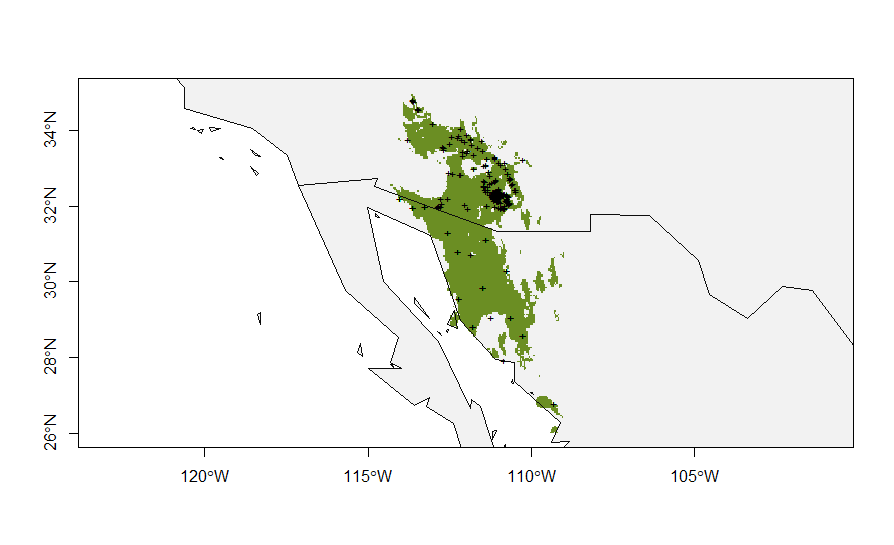
\includegraphics{/path/to/C:/Users/katca/Desktop/Reproducible_Science/SaguaroSDM_Image}
\caption{Caption for the picture.}
\end{figure}

\begin{center}\rule{0.5\linewidth}{\linethickness}\end{center}

\#Discussion

\begin{center}\rule{0.5\linewidth}{\linethickness}\end{center}

\#Citations
\url{https://www.wildflower.org/plants/result.php?id_plant=cagi10}

\end{document}
